%! TEX root = ../main.tex
\documentclass[../main.tex]{subfiles}

\begin{document}

\subsection{Fenditura $a = \qty{0.08}{\milli\metre}$}

\begin{figure}[ht!]
    \centering
    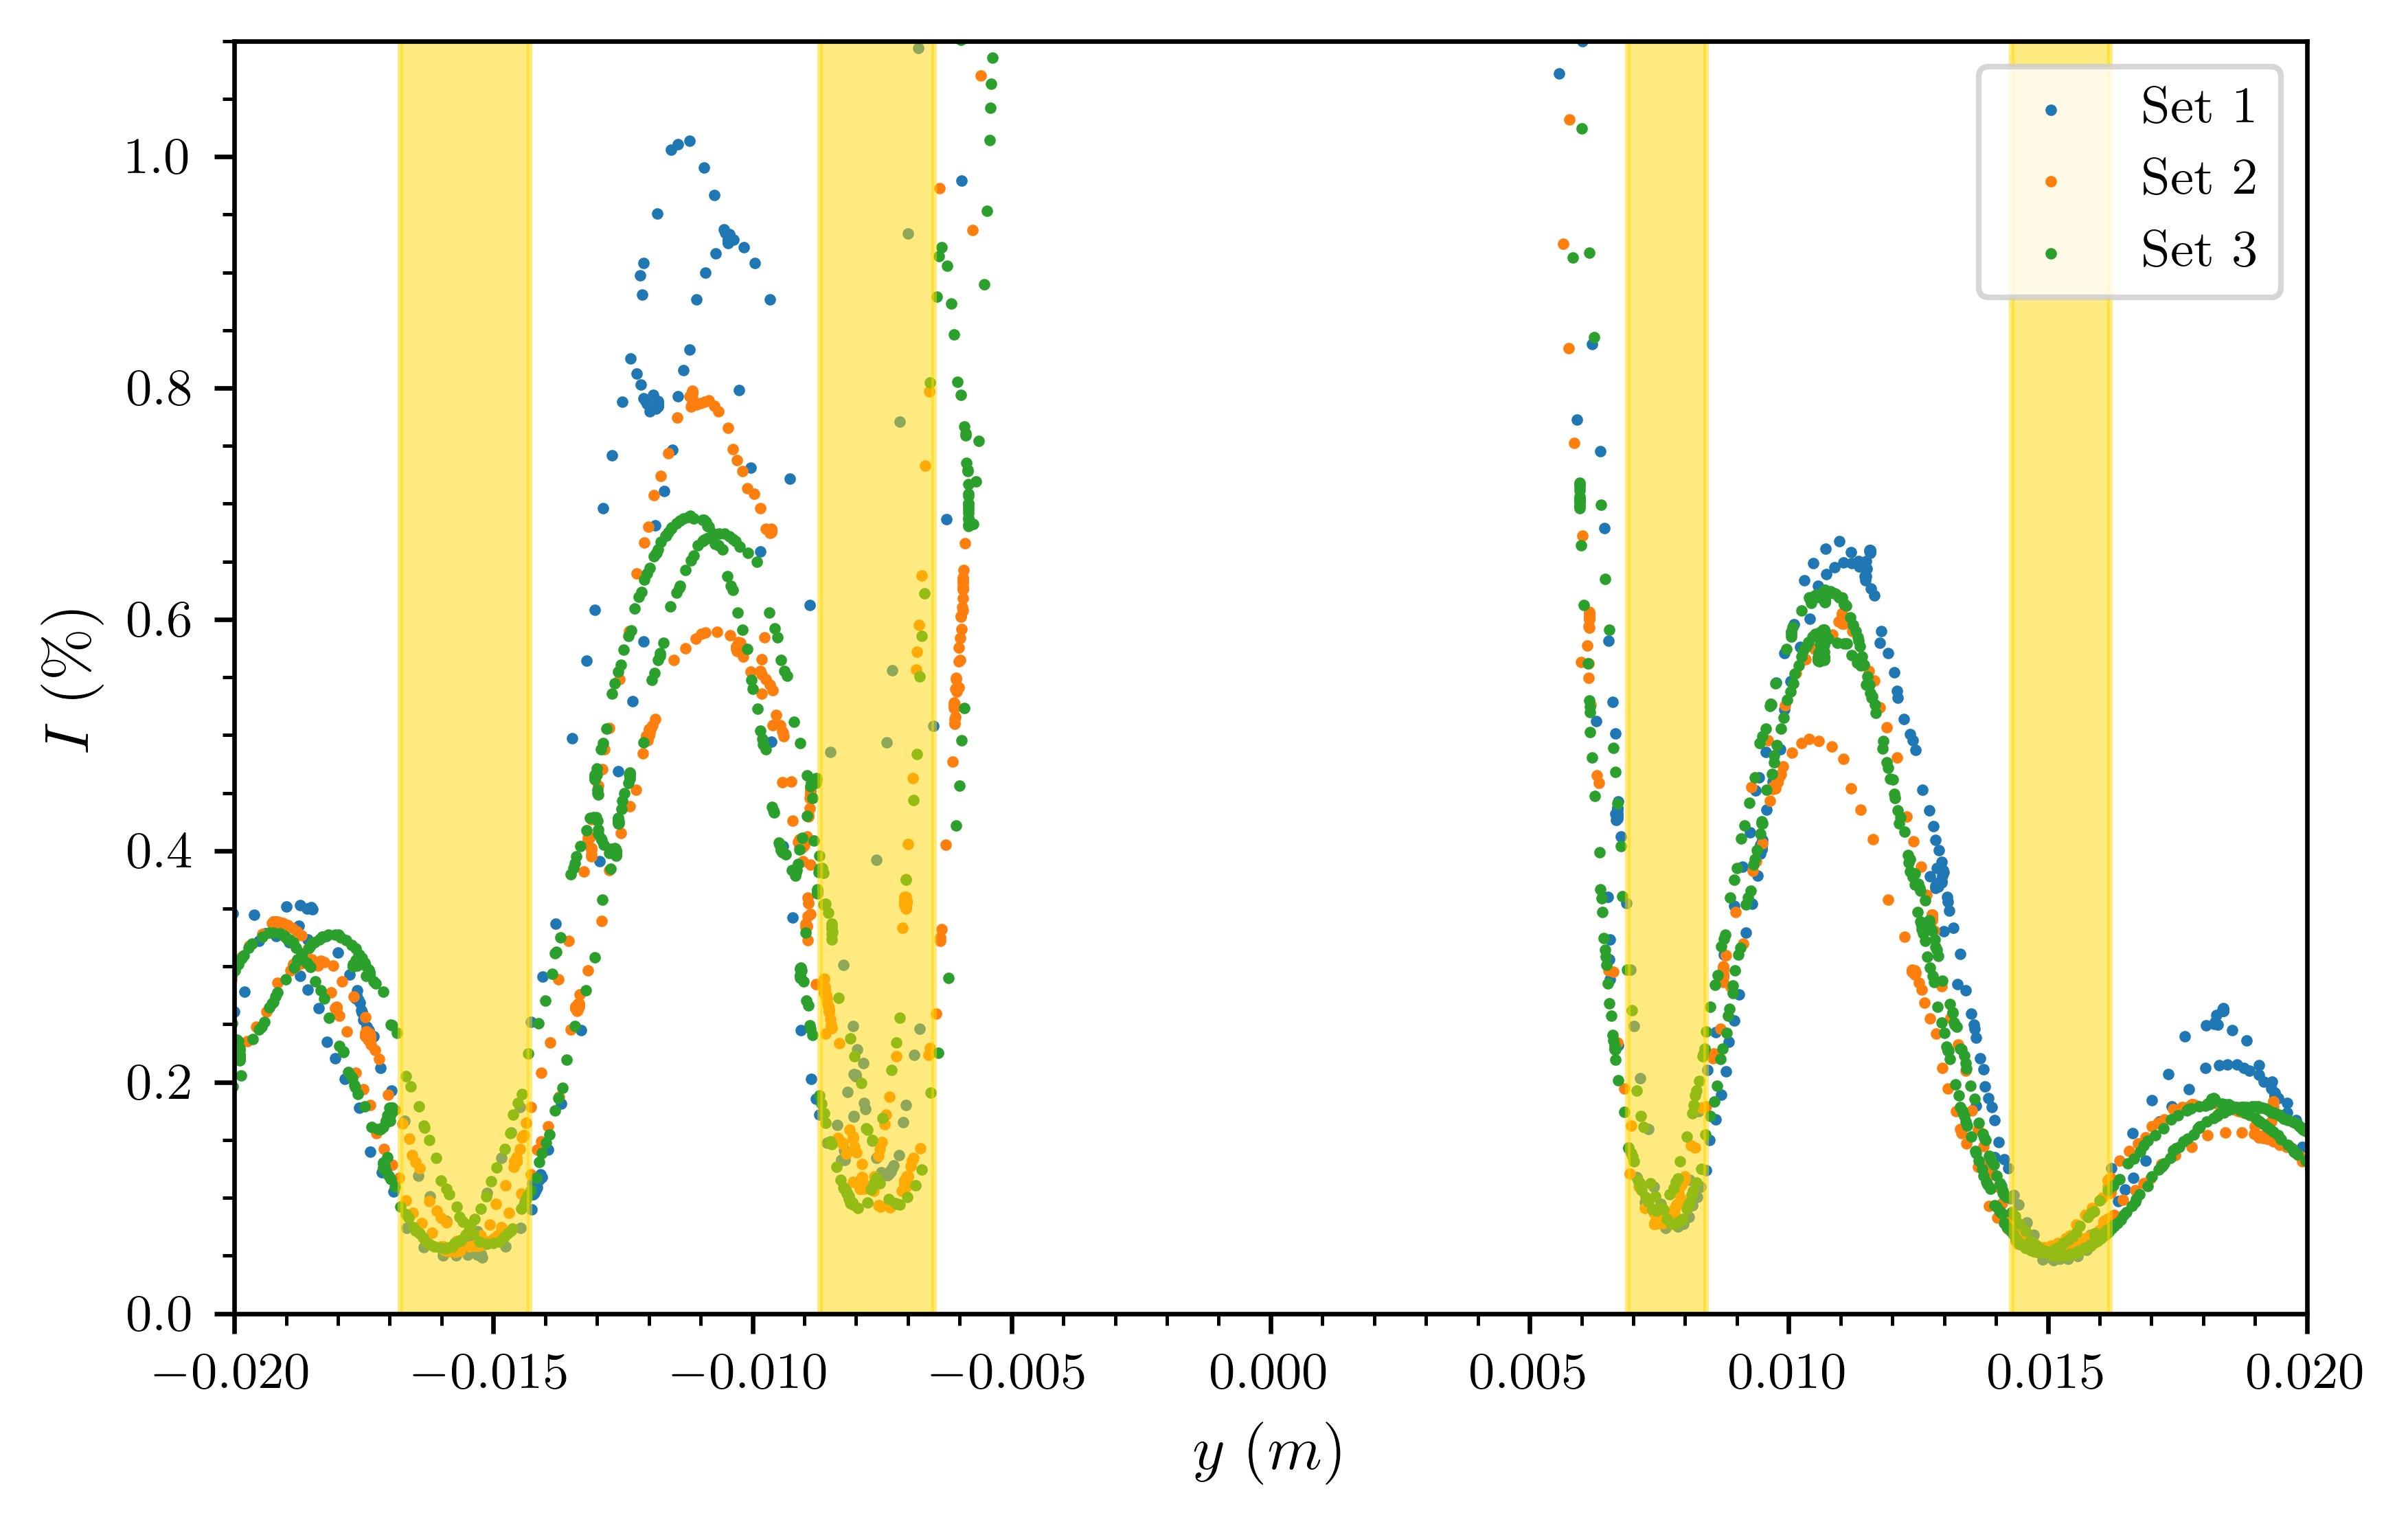
\includegraphics{min_0.08.png}
    \caption{Intensità luminosa $I$ in funzione della posizione $y$ del sensore (in metri) per la fenditura a $\qty{0.08}{\mm}$. I dati sono notevolmente asimmetrici, eccetto il set 3. In figura sono segnati i minimi ricavati graficamente con i relativi errori. Qui si considera un errore di posizione di $\qty{0.25}{\mm}$.} %todo: aggiungere qualcosa in più alla descrizione + commentare simmetria (o assenza) dei set
    \label{fig:minimi 0.08}
\end{figure}

\begin{table}[ht!]
    \centering
    \caption{}
    \import{../tables/}{mins_0.08.tex}
    \label{tab:minimi 0.08}
\end{table}

Intersecando i valori, si ottiene $a = 0.084 \pm 0.005$.

\begin{figure}[ht!]
    \centering
    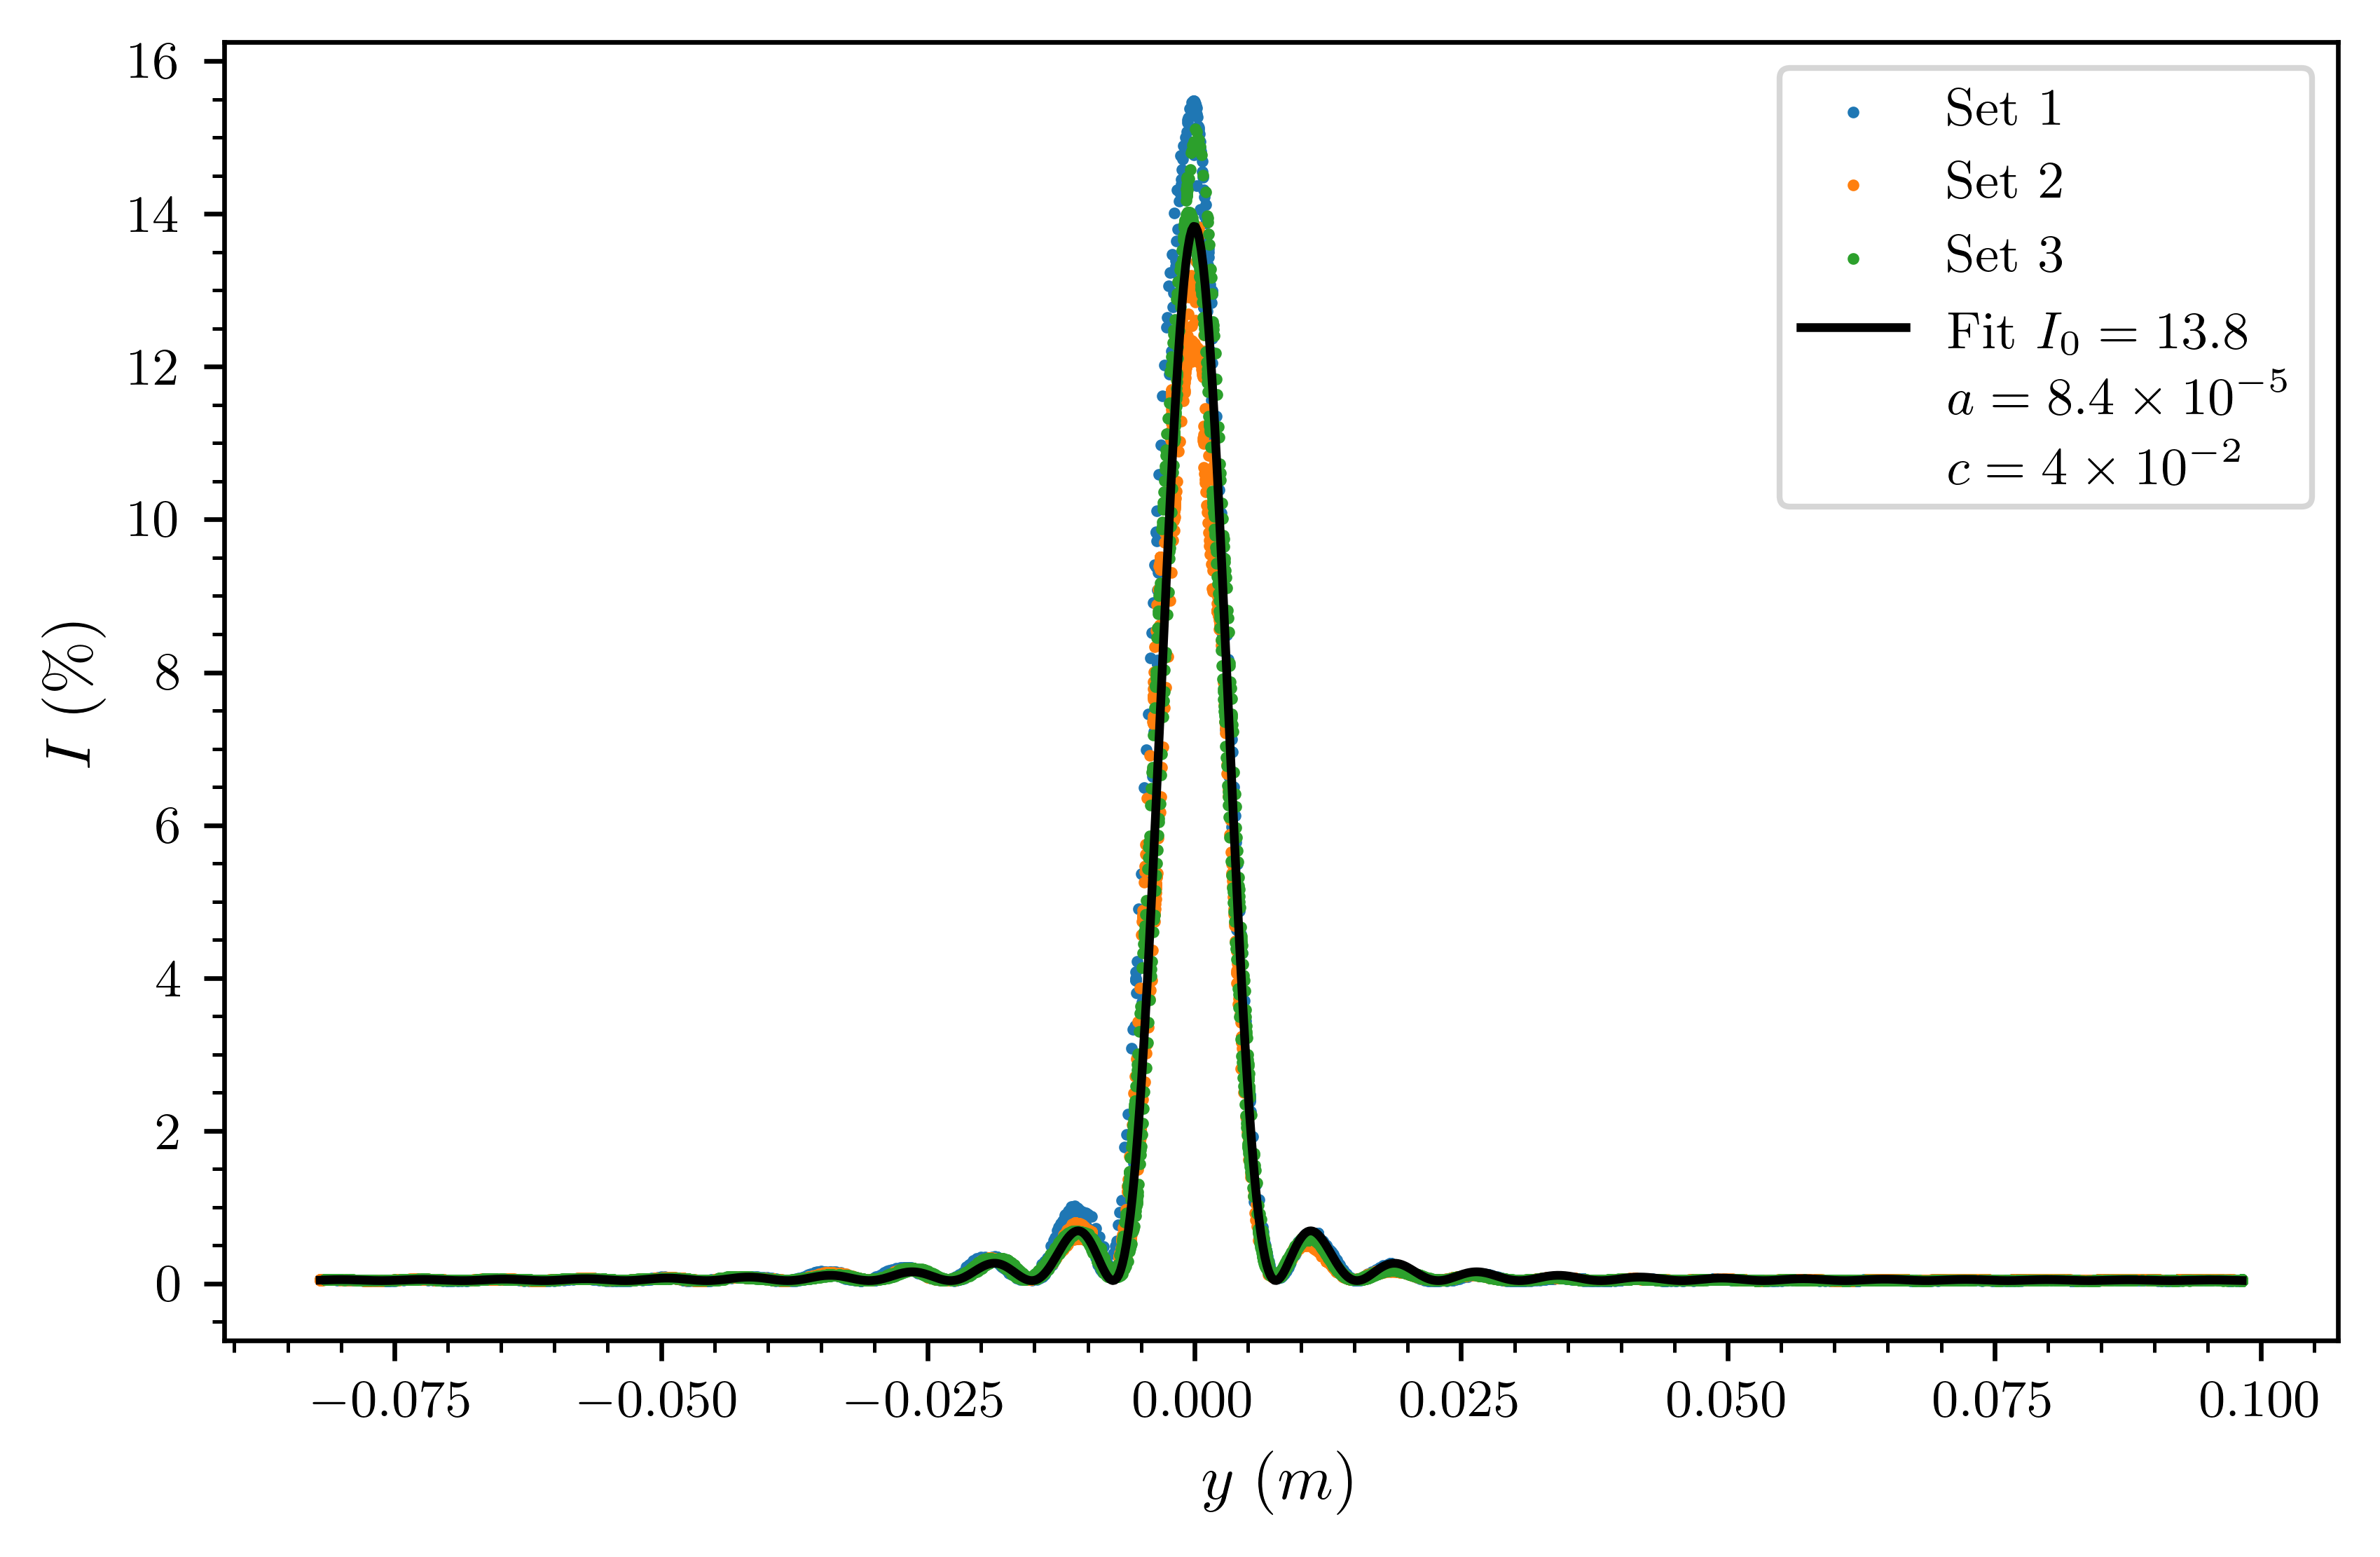
\includegraphics{fit_0.08.png}
    \caption{Intensità luminosa $I_{0}$ in funzione della posizione $y$ del sensore (in metri) per la fenditura a $\qty{0.08}{\mm}$. In figura è riportato il fit fatto utilizzando l'\autoref{eq:fit}. I valori dei parametri ottenuti sono $I_{0} = \num{13.8+-1.6}$, $a = \qty{8.4+-0.4e-5}{\mm}$ e $c = \num{4+-1.2e-2}$.}
    \label{fig:fit 0.08}
\end{figure}

I valori di $a$ ottenuti dal grafico e dal fit risultano compatibili con il valore teorico.

Anche qui si confrontano i dati ottenuti con ciascuna delle due aperture:

\begin{figure}[ht!]
    \centering
    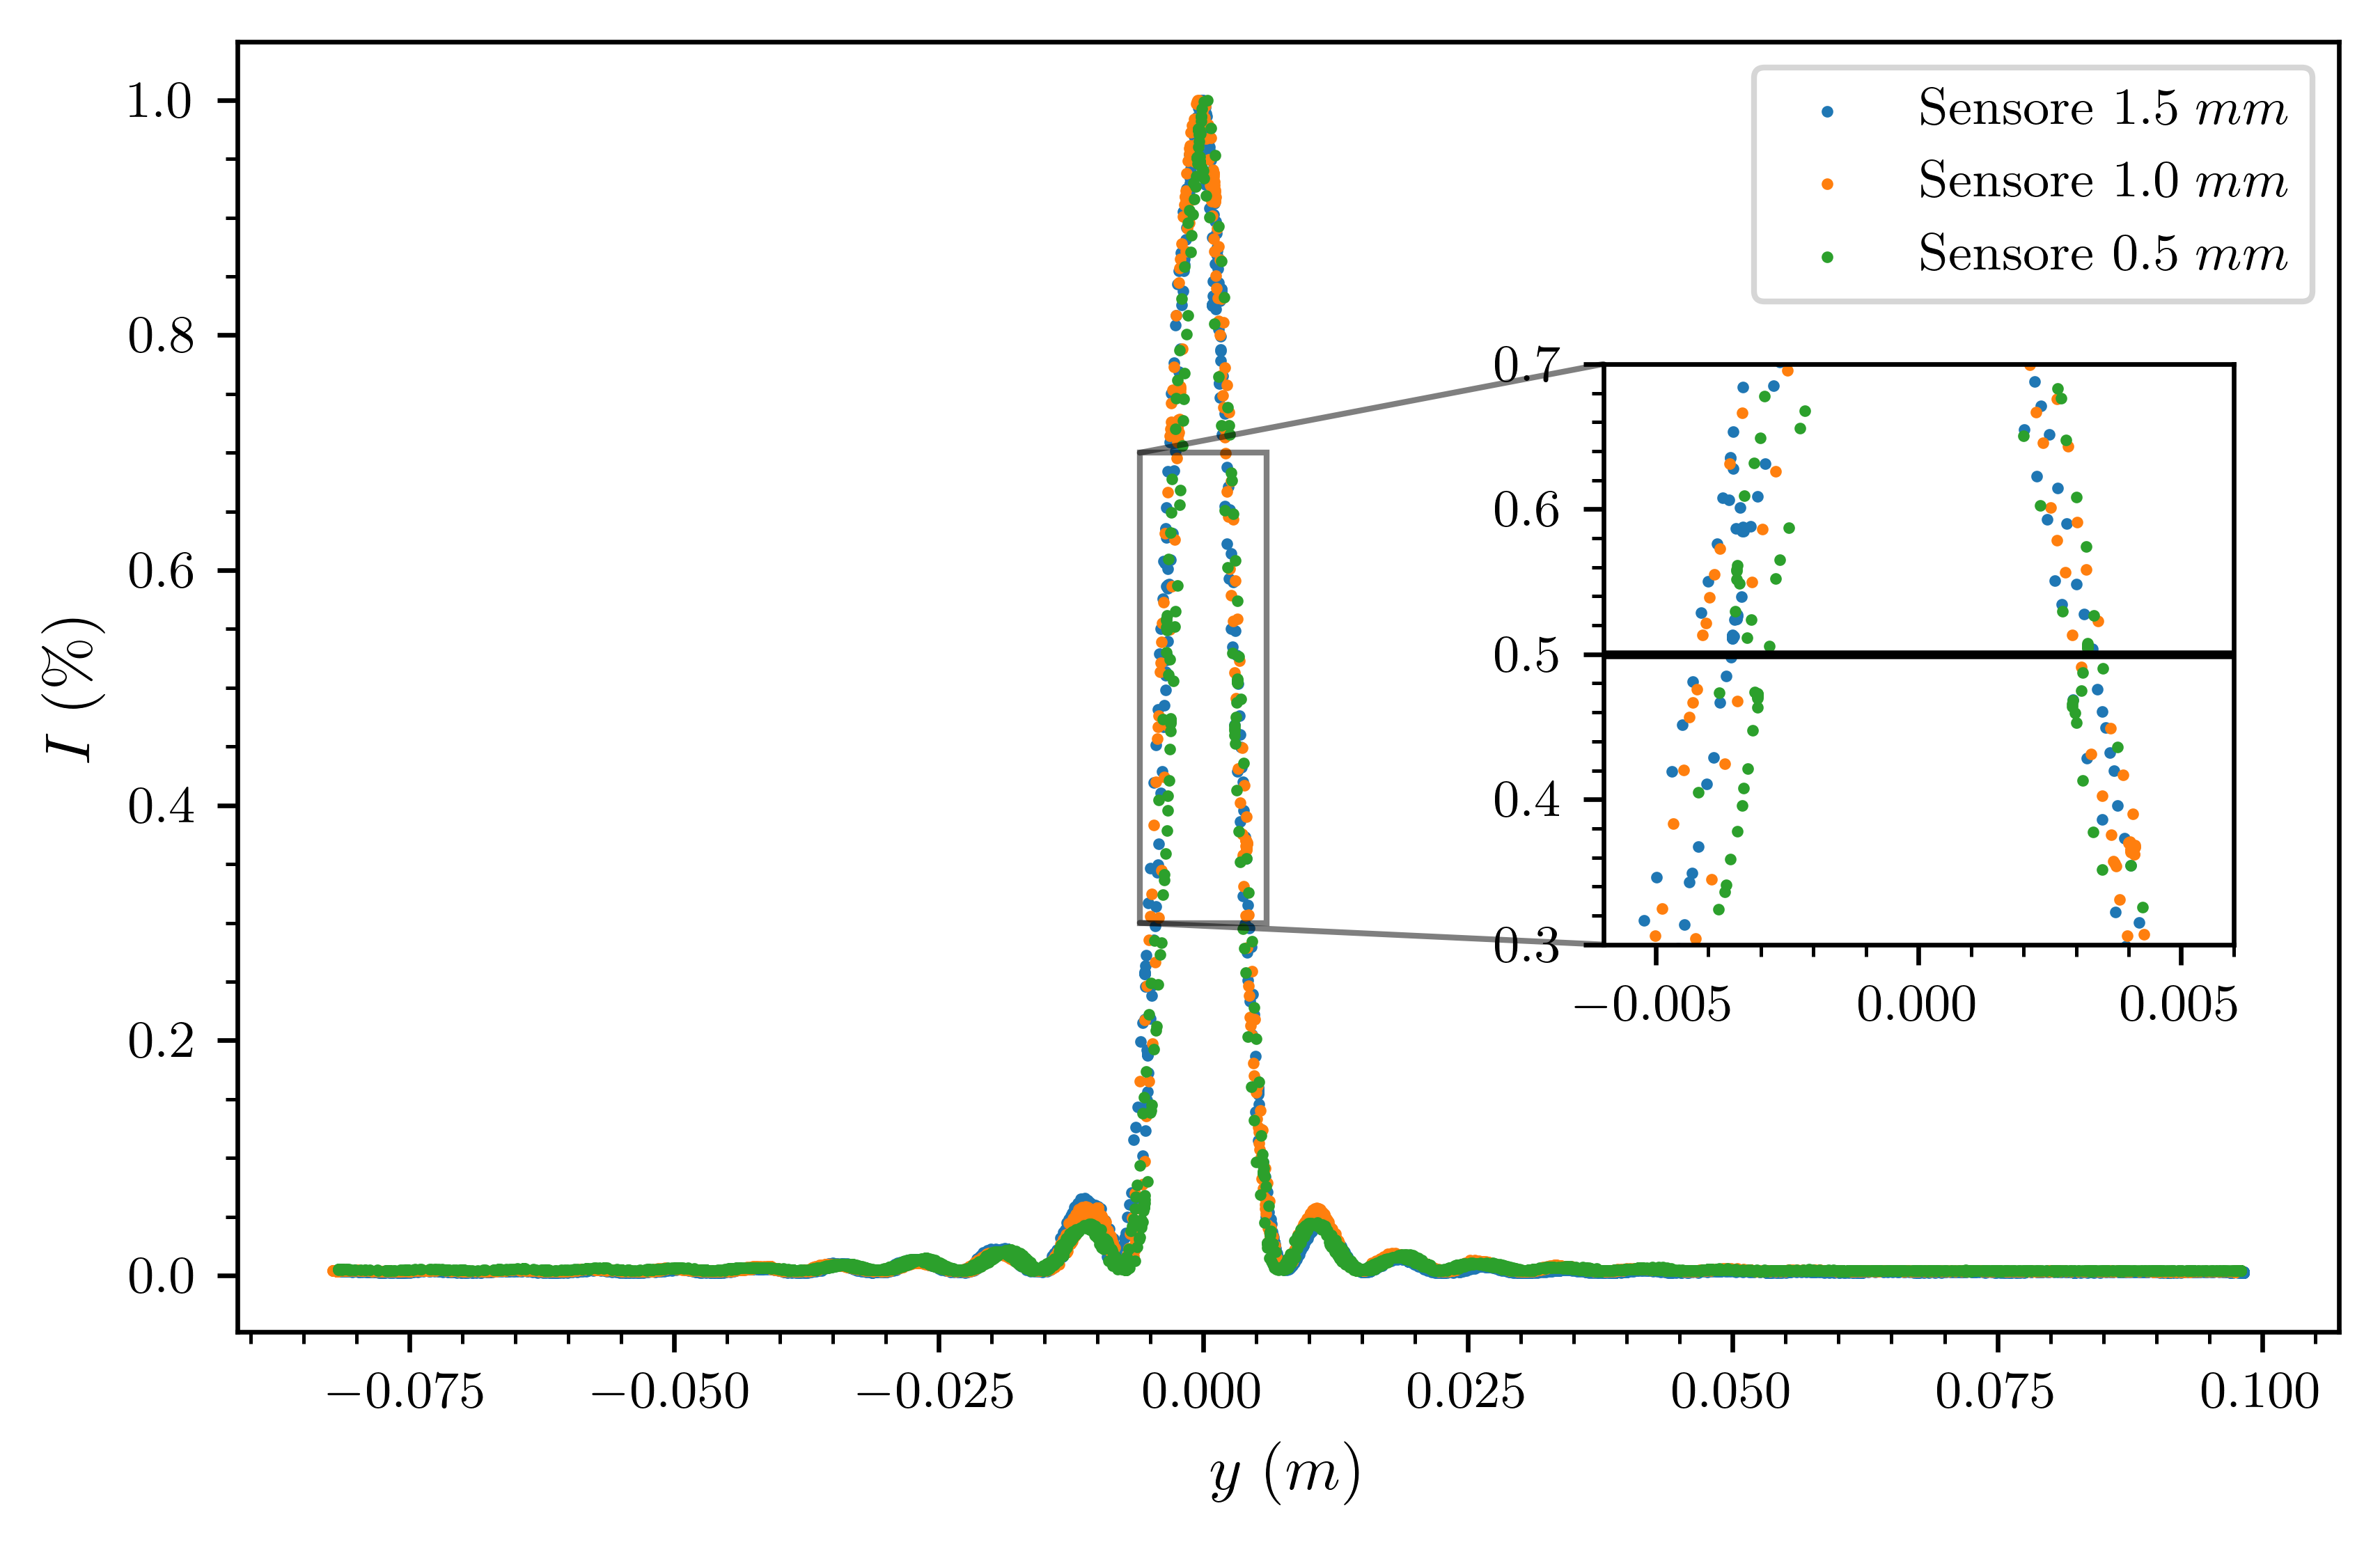
\includegraphics{sensor_0.08.png}
    \caption{}
    \label{fig:sensore 0.08}
\end{figure}

\end{document}